\documentclass[10pt]{beamer} %
\usetheme{Warsaw}
%\usetheme{CambridgeUS}
\usepackage[utf8]{inputenc}
\setbeamersize{text margin left=5mm,text margin right=5mm} 
%\usefonttheme{professionalfonts}
\usepackage{times}
\usepackage{verbatim}
\usepackage{tikz}
\usepackage{amsmath}
\usepackage{animate}
\usepackage{verbatim}
\usetikzlibrary{arrows,shapes}
\setbeamertemplate{navigation symbols}{}
\usefonttheme{serif}
%\usefonttheme[onlymath]{serif}
\usepackage{subfig}
\usepackage{framed}
\usepackage{amsmath}
\usepackage{amsfonts}
\usepackage{amssymb}
\usepackage{graphicx}
%\setbeamerfont{page number in head/foot}{size=\normalsize}
%\setbeamertemplate{footline}[frame number]
\usepackage{ifthen}
\usepackage{animate}
\newcommand*\oldmacro{}%
\let\oldmacro\insertshorttitle%
\renewcommand*\insertshorttitle{%
	\oldmacro\hfill%
	\insertframenumber\,/\,\inserttotalframenumber}
\setbeamercovered{transparent}
\usepackage{tikz}
\usetikzlibrary{calc}
\usepackage{pgfplots}
\usepackage{tikz-3dplot}
\usetikzlibrary{decorations.markings}
\usetikzlibrary{shapes,arrows}
\newcommand{\midarrowright}{\tikz \draw[-triangle 90] (0,0) -- +(.1,0);}
\newcommand{\midarrowup}{\tikz \draw[-triangle 90] (0,0) -- +(0,.1);}
%\usepackage{beamerthemesplit}
\setbeamertemplate{footline}
{%
	\leavevmode%
	\hbox{\begin{beamercolorbox}[wd=.13\paperwidth,ht=2.5ex,dp=1.125ex,leftskip=.3cm plus1fill,rightskip=.3cm]{author in head/foot}%
			\usebeamerfont{author in head/foot}\insertshortauthor
		\end{beamercolorbox}%
		\begin{beamercolorbox}[wd=.87\paperwidth,ht=2.5ex,dp=1.125ex,leftskip=.3cm,rightskip=.3cm plus1fil]{title in head/foot}%
			\usebeamerfont{title in head/foot}\insertshorttitle
	\end{beamercolorbox}}%
	\vskip0pt%
}


\usetikzlibrary{shadings, calc, decorations.markings, arrows, shapes}
\tikzset{->-/.style={decoration={
			markings,
			mark=at position #1 with {\arrow{<}}},postaction={decorate}},
	->-/.default=0.3,
}

\tikzset{->>-/.style={decoration={
			markings,
			mark=at position #1 with {\arrow{<}}},postaction={decorate}},
	->>-/.default=0.7,
}

\setbeamertemplate{headline}{}


\tikzset{
	invisible/.style={opacity=0},
	visible on/.style={alt={#1{}{invisible}}},
	alt/.code args={<#1>#2#3}{%
		\alt<#1>{\pgfkeysalso{#2}}{\pgfkeysalso{#3}} % \pgfkeysalso doesn't change the path
	},
}

\newcommand\ds{\displaystyle}
\newcommand\ts{\textstyle}
\newcommand{\mb}{\mathbf}
%\renewcommand{\thenotation}{}
%\renewcommand{\theequation}{\thesection.\arabic{equation}}
\def\Caption #1{\caption{\footnotesize #1}}
%\renewcommand\Caption{#1}{\Caption{\small{#1}}}
%\def\Caption #1{\Caption{\small{{#1}}}}

\def \Bfemph #1{\textbf{\emph{#1}}}


%\def\Proof.{{\medbreak\noindent{\it Dimostrazione}\enspace}}
\def\Proof{{\medbreak\noindent{\textbf{Proof.} }}}
\def\Proofsketch{{\medbreak\noindent{\textbf{Sketch of proof.} }}}
\def\endproof{~\hfill $\blacksquare$}
%\def\endproof{\hfill$\square$\par\medskip}

\def\Svolgimento{{\medbreak\noindent{\textit{Execution.} }}}
\def\Suggerimento{{\medbreak\noindent{\textit{Hint:} }}}



\usepackage{physics}
\usepackage[separate-uncertainty = true]{siunitx}
%\usepackage{amsmath} % or simply amstext
\newcommand{\angstrom}{\text{\normalfont\AA}}
\renewcommand{\si}[1]{\mathrm{#1}}


\renewcommand{\hat}[1]{\widehat{#1}}
\renewcommand{\theta}{\vartheta}
\renewcommand{\phi}{\varphi}
\renewcommand{\epsilon}{\varepsilon}
%\renewcommand{\phi}{\varphi}
\newcommand{\res}{\mathop{\mathrm{Res }}}
\newcommand{\red}[1]{\textcolor{red}{#1}}
%\newcommand{\blu}[1]{\textcolor{blue}{#1}}

\newcommand{\colonna}[2]{\begin{pmatrix}
		#1 \\ #2
\end{pmatrix}}
\newcommand{\riga}[2]{\begin{pmatrix}
		#1 & #2
\end{pmatrix}}
%%%%%%%%%%%%%%%%%%%%%%%%%%%%%%%%%%%%%%%%%%%%%%%%%%%%%%%%%%%%%%%%%%%%%%%%%%%%%%%%%%%%%%%%%%%




\usepackage{pgfplots}

\pgfplotsset{compat=newest}

%%\setbeamercovered{transparent}
%\setbeamertemplate{navigation symbols}{}
%%\setbeamercolor{block title}{use=structure,fg=white,bg=purple!75!black}
%\setbeamercolor{title}{use=structure,fg=red!75!black,bg=white!97!red,}
%\setbeamercolor{block title}{use=structure,bg=red!75!black,fg=white!97!red,}
%\setbeamercolor{block body}{use=structure,fg=black,bg=white!97!red,}


\author{Rubens Longhi}
\title[On the role of boundary conditions in the construction of fundamental solutions for Maxwell's eqns. on spacetimes with timelike boundary]{On the role of boundary conditions in the construction of fundamental solutions for Maxwell's equations on spacetimes with timelike boundary}
\date{September 24, 2019}

\AtBeginSection[]
{
	\begin{frame}[noframenumbering]
		\frametitle{Table of Contents}
		\tableofcontents[currentsection]
	\end{frame}
}
%\beamerdefaultoverlayspecification{<+->}


\usepackage{lipsum}

\newcommand\blfootnote[1]{%
	\begingroup
	\renewcommand\thefootnote{}\footnote{#1}%
	\addtocounter{footnote}{-1}%
	\endgroup
}

%\setbeamercolor{alerted text}{fg=blue}


\begin{document}




% For every picture that defines or uses external nodes, you'll have to
% apply the 'remember picture' style. To avoid some typing, we'll apply
% the style to all pictures.
\tikzstyle{every picture}+=[remember picture]

% By default all math in TikZ nodes are set in inline mode. Change this to
% displaystyle so that we don't get small fractions.
%\everymath{\displaystyle}

\begin{frame}
	\centering
	\includegraphics[width=0.2\textwidth]{unipv}\par\vspace{-0.4cm}
	\begin{center}
		\noindent%\fontsize{8pt}{\baselineskip}\selectfont
		\textsc{Universit\`a degli Studi di Pavia}
	\end{center}
\vspace{-0.6cm}
\begin{center}
	\begin{block}
		
		\begin{center}
			{\large \textcolor{blue!50!black}{\inserttitle}}
		\end{center}
		
	\end{block}
	
\end{center}

\vspace{-0.5cm}

\hfill	\begin{columns}[t]
	
	\begin{column}{.3\linewidth}
		
		
	%\vspace{.2cm}
%	\begin{flushleft}
		{\footnotesize Relatore:\\
			\textbf{Prof. Claudio Dappiaggi}\\[.3cm]} % Advisor's/supervisor's name
		{\footnotesize Correlatore:\\
			\textbf{Dott. Nicol\'o Drago}\\[.3cm]} % Advisor's/supervisor's name
%	\end{flushleft}
		
		
	\end{column}
	
	
	\begin{column}{.4\linewidth}
		\vspace{-0.3cm}
		\begin{flushright}
	{\footnotesize Tesi per la Laurea Magistrale di:\\ \textbf{Rubens Longhi}} % Text prior to the author name - right aligned and bold
		\end{flushright}
		
		
		
		
	\end{column}
	
	
\end{columns}

	
	




	
\end{frame}

\begin{frame}<beamer>
	\frametitle{Table of Contents}
	\tableofcontents
\end{frame}

\section{Introduction}


\begin{frame}
		\frametitle{Introduction (1)}
		
		This thesis deals with the characterization of the space of solutions of Maxwell's equations in terms of \red{Green functions} in spacetimes with timelike boundary. The aims are:
		\vskip0.5cm
		\begin{itemize}[<+-| alert@+>]
			\item Set Maxwell's equations in non-Minkowskian spacetimes with boundary\vskip0.25cm
			\item Prove existence and uniqueness of Green functions for $\Box$ with certain classes of boundary conditions\vskip0.25cm
			\item Construct the space of classical solutions for Maxwell's equations\vskip0.25cm
			\item Construct the classical and quantum algebra of observables of the system
		\end{itemize}
	%\pause
	\blfootnote{\scriptsize  C. Dappiaggi, N. Drago, and R.L. \emph{On Maxwell’s Equations
			on Globally Hyperbolic Spacetimes with Timelike Boundary.} In: arXiv:1908.09504 (2019)}
\end{frame}

\begin{frame}
\frametitle{Introduction (2)}

Applications to the study of several physical models in regions where the flux of physical quantities through the boundary is zero.\vskip0.5cm
\begin{columns}[t]
	
	\begin{column}{.55\linewidth}
		\begin{itemize}[<+-| alert@+>]
			\item Classical and quantum fields in curved spacetimes with boundary\vskip0.25cm
			\item Electromagnetic Casimir effect\vskip0.25cm
			\item Quantum Hall effect
		\end{itemize}
	\end{column}
	
	
	\begin{column}{.40\linewidth}
		
		%\vskip0.3cm
		\centering
		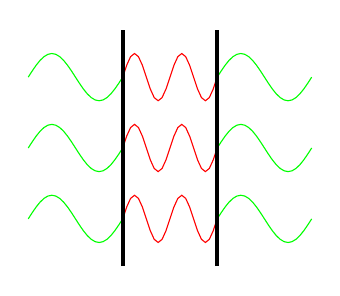
\begin{tikzpicture}[scale=0.6]
		\tikzstyle{every node}=[font=\scriptsize]
		
		\draw [domain=-1:1, red] plot (\x,{1.5+0.5*sin(2*pi*\x r)}) ;
		\draw [domain=-1:1, red] plot (\x,{-1.5+0.5*sin(2*pi*\x r)}) ;
		
		\draw [domain=1:3, green] plot (\x,{-1.5-0.5*sin(pi*\x r)}) ;
		\draw [domain=1:3, green] plot (\x,{1.5-0.5*sin(pi*\x r)}) ;
		
		\draw [domain=-3:-1, green] plot (\x,{-1.5-0.5*sin(pi*\x r)}) ;
		\draw [domain=-3:-1, green] plot (\x,{1.5-0.5*sin(pi*\x r)}) ;
		
		\draw [domain=-1:1, red] plot (\x,{0.5*sin(2*pi*\x r)}) ;
		\draw [domain=1:3, green] plot (\x,{-0.5*sin(pi*\x r)}) ;
		\draw [domain=-3:-1, green] plot (\x,{-0.5*sin(pi*\x r)}) ;
		
		\draw[ultra thick] (-1,-2.5) -- (-1,2.5);
		\draw[ultra thick] (1,-2.5) -- (1,2.5);
		
		\end{tikzpicture}
		
		
		
	\end{column}

\end{columns}



 
\end{frame}



\section{Spacetimes with timelike boundary}





\begin{frame}
\frametitle{Globally Hyperbolic Spacetimes with timelike boundary}
We consider \red{globally hyperbolic} spacetimes $M$, $\dim M=m\geq 2$ with \red{timelike boundary}.
\begin{block}{\textbf{Definition.}}
	A spacetime with boundary $(M,g)$ is globally hyperbolic if it is time-oriented, causal, and any causal diamond is compact\footnotemark.\\
	\vskip0.2cm
	$M$ has a timelike boundary if $\partial M$ is itself a time-oriented spacetime with the induced metric $\iota^*g$, $\iota:\partial M\to M$ being the immersion map.
\end{block}\footnotetext{\scriptsize for all $p,q\in M$ $J^+(p)\cap J^-(q)$ is compact, $J^\pm(p)$ being the future and past of the event $p$}\pause

\vskip-.5cm

\begin{columns}[t]
	
	\begin{column}{.50\linewidth}
		\begin{block}{\textbf{Theorem.}}
			$M$ can be split as $$M=\mathbb{R}\times\Sigma,$$ where $\Sigma$ is a Riemannian manifold with boundary $\partial \Sigma$.
		\end{block}
	\end{column}
	
	
	\begin{column}{.40\linewidth}
		
		\vskip0.3cm
		\centering
		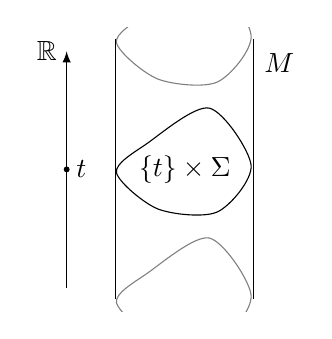
\begin{tikzpicture}[scale=0.6]
		
		\begin{scope}
		\clip (-1.5,-3) rectangle (1.5,3);
		
		\begin{scope}[shift={(0,2.75)}]
		\pgfmathsetseed{3}
		\draw[color=gray] plot [smooth cycle, samples=6,domain={1:6}] (\x*360/6+5*rnd:0.5cm+1cm*rnd);
		\end{scope}
		
		\begin{scope}[shift={(0,-2.75)}]
		\pgfmathsetseed{3}
		\draw[color=gray] plot [smooth cycle, samples=6,domain={1:6}] (\x*360/6+5*rnd:0.5cm+1cm*rnd);
		\end{scope}
		 
		\end{scope}
		
		
		\pgfmathsetseed{3}
		\draw plot [smooth cycle, samples=6,domain={1:6}] (\x*360/6+5*rnd:0.5cm+1cm*rnd) node at (0,0) {$\{t\}\times\Sigma$};
		\draw[] (-1.47,-2.75) -- (-1.47,2.75);
		\draw[] (1.45,-2.75) -- (1.45,2.75);
		\draw[-latex] (-2.5,-2.5) -- (-2.5,2.5) node[left] {$\mathbb{R}$};
		\draw[fill] (-2.5,0) circle (0.5mm) node[right]  {$t$};
		\node at (2,2.25) {$M$};
		\end{tikzpicture}
		
		
		
	\end{column}
	
\end{columns}




\end{frame}


\begin{frame}
	\frametitle{Static spacetimes}
	We restrict ourselves to \red{static} spacetimes:
	\begin{block}{\textbf{Definition.}}
		A globally hyperbolic spacetime with boundary $(M,g)$ is static if $\partial_t$ is global timelike irrotational vector field, i.e. $\mathcal{L}_{\partial_t}(g)=0$.
	\end{block}\pause
\vskip.5cm



\begin{columns}[t]
	
	\begin{column}{.60\linewidth}
		{ Examples:
			\begin{itemize}
				\item Half Minkowski spacetime $(\mathbb{R}^m_+=\mathbb{R}^{m-1}\times[0,+\infty),\eta)$
				\item Any globally hyperbolic sub-region with timelike boundary of Minkowski spacetime
				\item Non rotating black hole: exterior Schwarzschild spacetime (empty boundary)
%				$	 M=\mathbb{R}\times(2\mathrm{m},+\infty)	\times S^2	$  with metric {\footnotesize $g=-f(r) \mathrm{d} t^2+\frac{1}{f(r)} \mathrm{d} r^2	+r^2\,g_{S^2}$,}
%				where $f(r)=1-\frac{2\mathrm{m}}{r}$, $m\geq 0$.
		\end{itemize}}
	\end{column}
	
	
	\begin{column}{.40\linewidth}
		
		\vspace{-0.5cm}
		\centering
		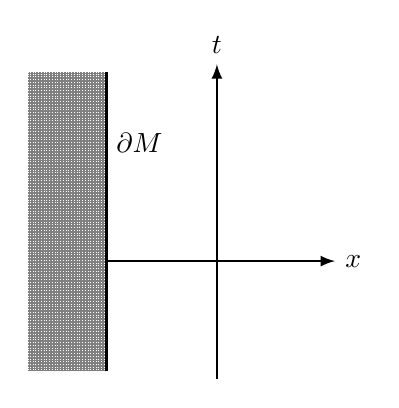
\begin{tikzpicture}
		
		%\draw[style=help lines, step=0.5, color=gray] (-0.9,-1.9) grid (1.9,1.9);
		\draw[style=help lines, step=0.02, color=gray] (-1.9,-1.9) grid (-0.9,1.9);
		%\draw[ color=green, -latex, decorate, decoration={snake, amplitude=0.4mm, segment length=2mm, post length=1mm}, segment aspect=0, very thick](0.5,-0.5) -- (-0.9,0.9);
		%\draw[ color=green, -latex, decorate, decoration={snake, amplitude=0.4mm, segment length=2mm, post length=1mm}, segment aspect=0, very thick] (-0.9,0.9) -- (0,1.8);
		
		\draw[-latex, thick] (-0.9,-0.5) -- (2,-0.5) node[right] {$x$};
		\draw[-latex, thick] (0.5,-2) -- (0.5,2) node[above] {$t$};
		\draw[very thick] (-0.9,-1.9) -- (-0.9,1.9);
		\node[right] at (-0.9, 1) {$\partial M$};
		
		\end{tikzpicture}
		
		
	\end{column}
	
\end{columns}


\end{frame}

\section{Green operators}


\begin{frame}
	\frametitle{Classical fields on spacetimes}
	Classical \red{fields} are solutions to partial differential equations of motion.
	
\vskip.3cm
	Examples:
	
\vskip.5cm
\begin{center}
	\begin{tabular}{cc}
		%\hline 
		Schroedinger field & $(i\partial_t-H)\psi=0$ \\ 
		\rule{0pt}{3ex}%\hline 
		Klein-Gordon field &  $(\Box+m^2)\phi=f$\\ 
		\rule{0pt}{3ex}%\hline 
		Dirac field &  $(i\gamma^\mu\partial_\mu-m)\psi=f$\\ 
		%\hline 
	\end{tabular}
\end{center}
 
\vskip.5cm
	
	\begin{columns}[t]
		
		\begin{column}{.60\linewidth}
			They are all of the form $P\psi=f$, where $P$ is a \red{differential operator} and $f\in C^\infty_{\mathrm{c}}(M)$ is an \red{external source}. We are interested in providing a solutions that propagates the signal from the source at \red{finite speed}.
		\end{column}
		
		
		\begin{column}{.35\linewidth}
			
			%\vspace{-0.5cm}
			\centering
			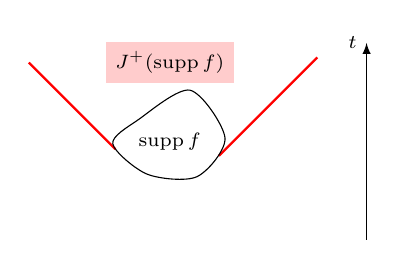
\begin{tikzpicture}[scale=0.5]
			
			\tikzstyle{every node}=[font=\scriptsize]
			\begin{scope}[shift={(1.25,-0.37)}]
			\draw[thick,red] (0,0) -- (2.5,2.5);
			\end{scope}
			
			\begin{scope}[shift={(-1.38,-0.2)}]
			\draw[thick, red] (0,0) -- (-2.2,2.2);
			\end{scope}
			
			\node[fill=red!20] at (0,2) {$J^+(\operatorname{supp} f)$};
			
%			\begin{scope}[shift={(1.25,0.47)}]
%			\draw[thick, blue] (0,0) -- (2.5,-2.5);
%			\end{scope}
%			
%			\begin{scope}[shift={(-1.38,0.1)}]
%			\draw[thick,blue] (0,0) -- (-2.2,-2.2);
%			\end{scope}
%			
%			\node[fill=blue!20] at (0,-2) {$J^-(\operatorname{supp} f)$};
			
			\draw[-latex] (5,-2.5) -- (5,2.5) node[left] {$t$};
			
			\pgfmathsetseed{3}
			\draw plot [smooth cycle, samples=6,domain={1:6}] (\x*360/6+5*rnd:0.5cm+1cm*rnd) node at (0,0) {$\operatorname{supp}f$};
			
			\end{tikzpicture}
			
			
		\end{column}
		
	\end{columns}
	
\end{frame}


\begin{frame}
	\frametitle{Green functions or Fundamental solutions}
	To solve $P\psi=f$ we look for the \red{inverses} of $P$, namely \red{fundamental solutions} or \red{Green operators} $G$. If a $G$ exists, it provides a solution of $P\psi=f$:
	\[	\psi=\operatorname{Id}\psi=GP\psi=G(\,f\,).	\]
	\vspace{-0.3cm}
	\begin{block}{\textbf{Definition.}}
		A Green operator $G:C^\infty_\mathrm{c}(M)\to C^\infty(M)$ for a differential operator $P$ is such that $G\circ P=\operatorname{Id}$, $P\circ G=\operatorname{Id}$.
	\end{block}
\vskip.4cm
\pause

We want to have the properties such that the propagation speed is \red{finite}.
\begin{columns}[t]
	
	\begin{column}{.50\linewidth}
		\begin{itemize}
			\item \red{advanced} Green operators \tikz[baseline]{
				\node[fill=red!20,anchor=base]
				{$G^+$};}, $\operatorname{supp}G^+(\,f)\subseteq J^+(\operatorname{supp} f)$
			\item \red{retarded} Green operators \tikz[baseline]{ \node[fill=blue!20,anchor=base]
			{$G^-$};}, $\operatorname{supp}G^-(\,f)\subseteq J^-(\operatorname{supp} f)$
		\end{itemize}
	\end{column}
	
	
	\begin{column}{.45\linewidth}
		
		\vspace{-0.3cm}
		\centering
		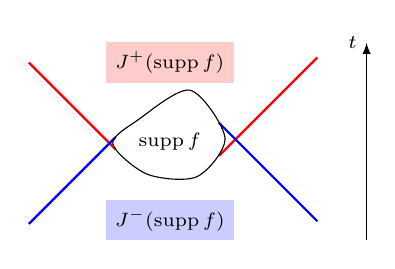
\begin{tikzpicture}[scale=0.5]
		
		\tikzstyle{every node}=[font=\scriptsize]
		\begin{scope}[shift={(1.25,-0.37)}]
		\draw[thick,red] (0,0) -- (2.5,2.5);
		\end{scope}
		
		\begin{scope}[shift={(-1.38,-0.2)}]
		\draw[thick, red] (0,0) -- (-2.2,2.2);
		\end{scope}
		
		\node[fill=red!20] at (0,2) {$J^+(\operatorname{supp} f)$};
		
		\begin{scope}[shift={(1.25,0.47)}]
		\draw[thick, blue] (0,0) -- (2.5,-2.5);
		\end{scope}
		
		\begin{scope}[shift={(-1.38,0.1)}]
		\draw[thick,blue] (0,0) -- (-2.2,-2.2);
		\end{scope}
		
		\node[fill=blue!20] at (0,-2) {$J^-(\operatorname{supp} f)$};
		
		\draw[-latex] (5,-2.5) -- (5,2.5) node[left] {$t$};
		
	\pgfmathsetseed{3}
	\draw plot [smooth cycle, samples=6,domain={1:6}] (\x*360/6+5*rnd:0.5cm+1cm*rnd) node at (0,0) {$\operatorname{supp}f$};
		
		\end{tikzpicture}
		
		
	\end{column}
	
\end{columns}
\vskip.2cm\pause
With $G^\pm$ we can construct \red{causal propagator} $G=G^+-G^-$.
	
\end{frame}

\section{Maxwell's equations}


\begin{frame}
	\frametitle{Differential forms and Maxwell's equations (1)}
	{ We denote the space of smooth \red{differential $k$-forms} over $M$ as $\Omega^k(M)$, $0\leq k\leq m$.\\
		\vskip.3cm
		
	Electromagnetic field is regarded as the \red{Faraday} $2$-form $F\in \Omega^2(M)$ (anti-symmetric covariant $2$-tensor).}\\
\vskip.3cm

	In terms of \red{electric} and \red{magnetic} fields it holds
			$\quad	F=B+\mathrm{d}t\wedge E,	$\\
			\vskip.13cm
		with $E\in C^\infty(\mathbb{R},\Omega^1(\Sigma))$ and $B\in C^\infty(\mathbb{R},\Omega^2(\Sigma))$.
		\vskip.1cm\pause
		
		\begin{block}{Maxwell's equations for $F$}
			Let $J\in\delta\Omega^2(M)$ be a $4$-current. Then Maxwell's equations for the Faraday tensor $F\in\Omega^2(M)$ are
			\[	\mathrm{d}F=0,\qquad \delta F=-J,		\]
			where $\mathrm{d}:\Omega^k(M)\to\Omega^{k+1}(M)$ and $\delta:\Omega^k(M)\to\Omega^{k-1}(M)$ are the \red{differential} and \red{codifferential} operators.
		\end{block}
	

	

	
\end{frame}

\begin{frame}
\frametitle{Differential forms and Maxwell's equations (2)}
\begin{block}{}
	\vspace{-0.2cm}
	\[	\mathrm{d}^2\omega=0,\quad \mathrm{\delta}^2\omega=0,\ \forall \omega\in\Omega^k(M).		\]
\end{block}

In empty space $J=0$ and $F$ is \red{closed} ($\mathrm{d}F=0$) and \red{co-closed} ($\delta F=0$).\\
\vskip.2cm
In local components one recovers the usual \red{covariant} expressions

\[	(\mathrm{d}F)_{ijk}=\partial_i F_{jk}+\partial_j F_{ki}+\partial_k F_{ij}=0,\quad 1\leq i,j,k\leq 4,		\]

\[	(\delta F)_k=\partial^{\,j}F_{jk}=0,\quad 1\leq k\leq 4.		\]\pause
 In \red{curved backgrounds} one has to add to the usual derivatives curvature some symmetric corrections $\Gamma$:
 \[	\partial\longrightarrow \partial+\Gamma=:\nabla	\]
 Since differential forms are totally anti-symmetric, the corrections are canceled.
 \begin{block}{}
 	Maxwell's equations are \red{invariant} in form in any curved spacetime: $$\mathrm{d}F=0,\qquad \delta F=-J.$$
 \end{block}
 


\end{frame}


\begin{frame}
	\frametitle{Maxwell's equations for the potential $A$ (1)}
	
	As a \red{gauge theory}, electromagnetism is formulated in terms of the potential $A\in\Omega^1(M)$. We look for a local primitive $A$ of $F$, i.e. $$F=\mathrm{d}A,\quad F_{ij}=\partial_iA_j-\partial_jA_i.$$
	
	The Faraday tensor $F\in\Omega^2(M)$ is \red{closed} ($\mathrm{d}F=0$), but not always \red{exact} ($F=\mathrm{d}A$), depending on the topology of $M$.
	



\begin{columns}[t]
	
	\begin{column}{.50\linewidth}
		\begin{block}{Aharonov-Bohm Effect}
		Consider $M$ as the exterior of a solenoid run by an electric current. There is no field ($F=0$), but $A\neq 0$ and $\mathrm{d}A=F=0$ only locally since the space is not \red{simply connected}.
		\end{block}
	\end{column}
	
	
	\begin{column}{.50\linewidth}
		
		\vspace{0.3cm}
		\centering
		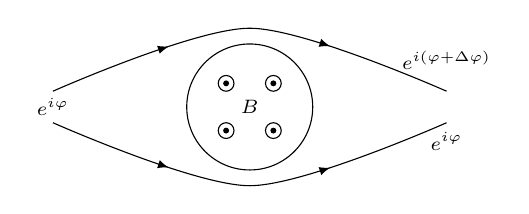
\begin{tikzpicture}%[scale=0.5]
		
		\tikzstyle{every node}=[font=\scriptsize]
		\draw (0,0) circle (0.8cm);
		\draw (0.3,0.3) circle (.1cm);
		\draw[fill] (0.3,0.3) circle (.03cm);
		
		\draw (-0.3,0.3) circle (.1cm);
		\draw[fill] (-0.3,0.3) circle (.03cm);
		
		\draw (0.3,-0.3) circle (.1cm);
		\draw[fill] (0.3,-0.3) circle (.03cm);
		
		\draw (-0.3,-0.3) circle (.1cm);
		\draw[fill] (-0.3,-0.3) circle (.03cm);
		
		\node at (0,0) {$B$};
		
		\begin{scope}[decoration={
			markings,
			mark=at position 0.3 with {\arrow{latex}}, mark=at position 0.7 with {\arrow{latex}}}
		]
		\draw[postaction={decorate}] plot [smooth] coordinates {(-2.5,0.2) (0,1) (2.5,0.2) };
		\end{scope}
		
		\begin{scope}[decoration={
			markings,
			mark=at position 0.3 with {\arrow{latex}}, mark=at position 0.7 with {\arrow{latex}}}
		]
		\draw[postaction={decorate}] plot [smooth] coordinates {(-2.5,-0.2) (0,-1) (2.5,-.2) };
		\end{scope}
		
		\node at (-2.5,0) {$e^{i\phi}$};
		
		\node[above] at (2.5,0.35) {$e^{i(\phi+\Delta\phi)}$};
		\node[below] at (2.5,-.2) {$e^{i\phi}$};
		
		
		
		\end{tikzpicture}
		
		
	\end{column}
	
\end{columns}
	
\end{frame}


\begin{frame}
	\frametitle{Maxwell's equations for the potential $A$ (2)}
	
	$F=\mathrm{d}A$ implies $\mathrm{d}F=\mathrm{d}^2A=0$ and $\delta F=\delta\mathrm{d}A=-J$.
	
	\begin{block}{Maxwell's equations for $A\in\Omega^1(M)$}
			\begin{equation}\label{Eqn: Maxwell A}
				\delta\mathrm{d}A=-J.
			\end{equation}	
	\end{block}
\vskip.3cm
	If $A'=A+\mathrm{d}\chi$, $\chi\in C^\infty(M)$: $\quad F_{A'}=\mathrm{d}A'=\mathrm{d}A+\mathrm{d}^2\chi=\mathrm{d}A=F_A$
	
	\begin{block}{Definition. (Gauge invariance with empty boundary)}
		If $\partial M=\emptyset$, $\ A,A'\in\Omega^1(M)$ solutions of \eqref{Eqn: Maxwell A} are \red{gauge-equivalent} if there exists $\chi\in C^\infty(M)$ such that $$A'=A+\mathrm{d}\chi.$$ Then $A\to A+\mathrm{d}\chi$ is called \red{gauge transformation}.
	\end{block}
	
\end{frame}

\begin{frame}
	\frametitle{Maxwell's equations for the potential $A$ (3)}
	
	
	Is there a gauge transformation $A\to A'$ such that $\Box A'=-J$, where $\Box=\delta\mathrm{d}+\mathrm{d}\delta$ is the wave operator?
	
 In \red{Lorenz gauge} $ \delta A'=0\,\Rightarrow\, \mathrm{d}\delta A'=0 \,\Rightarrow \,	(\delta\mathrm{d}+\mathrm{d}\delta)A'\!=\Box A'=-J$.
 
 \vskip.4cm

	The transformation $A\to A'=A+\mathrm{d}\chi$ must be such that $$\delta A'=\delta A+\delta\mathrm{d}\chi=\delta A+\Box\chi=0$$
	
	\begin{block}{}
		If $\partial M=\emptyset$, for any fixed $A\in\Omega^1(M)$ the equation $\Box\chi=-\delta A$ is always solvable.
	\end{block}

	\begin{block}{Theorem.}
	If $\partial M=\emptyset$, for any solution $A\in\Omega^1(M)$ there exists $A'\in\Omega^1(M)$ gauge equivalent to $A$ such that $A'$ satisfies the \red{Lorenz gauge} $\delta A'=0$ ($\partial^k\!A_k=0$) and hence the system becomes
	\vspace{-.1cm}
	\[	\Box A'=-J,\quad \delta A'=0.	\]
\end{block}
	
	
\end{frame}


\begin{frame}
	\frametitle{Green operators for $\Box$ with empty boundary}
	
	\begin{block}{Theorem.}
		If $M$ is globally hyperbolic with $\partial M=\emptyset$, there exist unique \red{advanced} and \red{retarded} Green operators $G^\pm$ for $\Box$.
	\end{block}

Solutions to Maxwell's equations are completely determined in terms of Green operators for $\Box$.
\[	A=\operatorname{Id}A=(G^\pm\circ \Box) A=-G^\pm (J).	\]\pause

Lorenz gauge is \red{preserved} since $\delta\circ G^\pm=G^\pm\circ\delta$:

$$\delta A=-\delta G(J)=-G(\delta J)=0,$$

with $\delta J=0$ being the conservation of current ($\partial_j J^j=0$).

\begin{block}{}
	In spacetimes with non-empty boundary $\delta\circ G^\pm=G^\pm\circ\delta$ can no longer hold depending on the \red{boundary conditions}.
\end{block}

	
	
\end{frame}


\section{Boundary conditions for $\Box$}

\begin{frame}
	\frametitle{Generalization to spacetimes with boundary}
	In spacetimes with non-empty boundary it is not always possible to solve $\Box\chi=-\delta A$.	We look for \red{boundary conditions} for $\Box$ such that $G^\pm$ exist.\\
	\vskip.2cm
	
\red{Physically sound} boundary conditions are those such that the flux of physical quantities vanish:
	
	\begin{block}{}
		We require the \red{symplectic flux} through the boundary to vanish (symmetric operator):
		$$\sigma(\alpha,\beta)=(\Box\alpha,\beta)-(\alpha,\Box\beta)=0,$$
		$\forall\alpha,\beta\in\Omega^1(M)$, $\operatorname{supp}\alpha\cap\operatorname{supp}\beta$ compact. $(\alpha,\beta)=\int_{M} \overline{\alpha}\wedge\star\beta=\int_{M}\overline{\alpha_j}\beta^j\,\mathrm{d}\mu_g,$
	\end{block}



\pause

\begin{columns}[t]
	
	\begin{column}{.65\linewidth}
	$$\sigma(\alpha,\beta)=
	(\mathrm{t}\delta\alpha,\mathrm{n}\beta)_\partial-
	(\mathrm{n}\alpha,\mathrm{t}\delta\beta)_\partial-
	(\mathrm{n}\mathrm{d}\alpha,\mathrm{t}\beta)_\partial+
	(\mathrm{t}\alpha,\mathrm{n}\mathrm{d}\beta)_\partial,$$
	
	Where for $\omega\in\Omega^1(M)$, $\mathrm{t}\omega$ is the projection on $\partial M$ and $\mathrm{n}\omega$ is the projection on the normal to $\partial M$.
	\end{column}
	
	
	\begin{column}{.30\linewidth}
		
	%	\vspace{-0.5cm}
		\centering
		\hspace{0.3cm}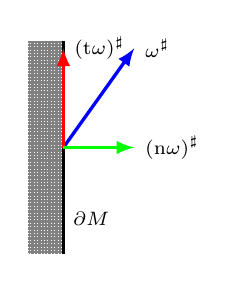
\begin{tikzpicture}[scale=0.9]
		
		\tikzstyle{every node}=[font=\scriptsize]
		
		%\draw[style=help lines, step=0.5, color=gray] (-0.9,-1.9) grid (1.9,1.9);
		\draw[style=help lines, step=0.02, color=gray] (-0.5,-1.5) grid (0,1.5);
		%\draw[ color=green, -latex, decorate, decoration={snake, amplitude=0.4mm, segment length=2mm, post length=1mm}, segment aspect=0, very thick](0.5,-0.5) -- (-0.9,0.9);
		%\draw[ color=green, -latex, decorate, decoration={snake, amplitude=0.4mm, segment length=2mm, post length=1mm}, segment aspect=0, very thick] (-0.9,0.9) -- (0,1.8);
		
		%\draw[-latex, thick] (-0.9,-0.5) -- (2,-0.5) node[right] {$x$};
		%\draw[-latex, thick] (0.5,-2) -- (0.5,2) node[above] {$t$};
		\draw[very thick] (-0,-1.5) -- (-0,1.5);
		\node[right] at (-0, -1) {$\partial M$};
		
		\draw[-latex, blue, very thick] (0,0) -- (1,1.4) node[black, right] {$\omega^\sharp$};
		
		\draw[-latex, red, very thick] (0,0) -- (0,1.4) node[black,right] {$(\mathrm{t}\omega)^\sharp$};
		
		\draw[-latex, green, very thick] (0,0) -- (1,0) node[black, right] {$(\mathrm{n}\omega)^\sharp$};
		
		\end{tikzpicture}
		
		
	\end{column}
	
\end{columns}
	
\end{frame}


\begin{frame}
	\frametitle{Boundary conditions for $\Box$}
	\begin{block}{Symplectic Flux}
		$$\sigma(\alpha,\beta)=
		(\mathrm{t}\delta\alpha,\mathrm{n}\beta)_\partial-
		(\mathrm{n}\alpha,\mathrm{t}\delta\beta)_\partial-
		(\mathrm{n}\mathrm{d}\alpha,\mathrm{t}\beta)_\partial+
		(\mathrm{t}\alpha,\mathrm{n}\mathrm{d}\beta)_\partial.$$
	\end{block}
	
	The symplectic flux vanishes if $\alpha,\beta$ are in the following spaces.\\
	
	\vskip.3cm
	We studied, among the others:
	
	\begin{itemize}[<+-| alert@+>]
		\item space of $k$-forms with {\em Dirichlet} boundary condition
		\begin{align*}
		\Omega^k_{\mathrm{D}}(M)\doteq\{\omega\in\Omega^k(M)\;|\;\mathrm{t}\omega=0\;,\;\mathrm{n}\omega=0\}\,,
		\end{align*}
		\item space of $k$-forms with {\em $\Box$-tangential} boundary condition
		\begin{align*}
		\Omega^k_\parallel(M)\doteq\{\omega\in\Omega^k(M)\;|\;\mathrm{t}\omega=0\;,\;\mathrm{t}\delta\omega=0\}\,,
		\end{align*}
		\item space of $k$-forms with {\em $\Box$-normal} boundary condition
		\begin{align*}
		\Omega^k_\perp(M)\doteq\{\omega\in\Omega^k(M)\;|\;\mathrm{n}\omega=0\;,\;\mathrm{nd}\omega=0\}\,.
		\end{align*}
	\end{itemize}
	
	
	
\end{frame}




\begin{frame}
	\frametitle{Splitting of $\Box$ in static spacetimes}
	
	In \red{static} globally hyperbolic spacetimes it holds $M=\mathbb{R}\times\Sigma$ and $\Box$ splits as
	\[	\Box=\partial^2_t-\Delta,		\]
	where $\Delta$ is the spatial Laplacian on $\Sigma$.\\
	\vskip.2cm\pause
	Since our boundary conditions are themselves \red{static}, the flux can be expressed with respect to the spatial derivatives only:
	$$\sigma(\alpha,\beta)=\left(\Delta(\alpha|_\Sigma),\beta|_\Sigma\right)_\Sigma-\left(\alpha|_\Sigma,\Delta(\beta|_\Sigma)\right)_\Sigma,$$
	where $(\,,\,)_\Sigma$ is the \red{Hilbert} scalar product in $\mathrm{L}^2\Omega^k(\Sigma)$.\pause
	\vskip.2cm
	\begin{block}{}
		Vanishing symplectic flux is equivalent to $\Delta$ being symmetric as a densely defined operator on $\mathrm{L}^2\Omega^k(\Sigma)$. For a \red{unitary} time evolution we look for a \red{self-adjoint} extension of $\Delta$.
	\end{block}
\vskip.2cm
To select self-adjoint extensions we use the method of \red{boundary triples.}
	
\end{frame}

\section{Boundary triples for $\Box$}

\begin{frame}
	\frametitle{Boundary triples (1)}
	\begin{block}{Definition.}
		A \red{boundary triple} for a symmetric differential operator $S$ on a Riemannian manifold with boundary $\Sigma$ is a triple $(\mathrm{L}^2\Omega^k(\partial\Sigma), \gamma_0,\gamma_1)$ such that $$\sigma(\alpha,\beta)=(\gamma_1 \alpha,\gamma_0\beta)_{\partial}-(\gamma_0 \alpha,\gamma_1\beta)_{\partial}$$ for any $\alpha,\beta\in\operatorname{dom}(S^*)$.
	\end{block}
\vskip.3cm
\red{Self-adjoint extensions} of $S$ are in one-to-one correspondence with all physically sound \red{boundary conditions}.\\
\vskip.3cm
The space $\ker(\mathcal{A}\gamma_1-\mathcal{B}\gamma_0)$ parametrizes the boundary conditions that vanish the symplectic flux, where $\mathcal{A,B}$ is a self-adjoint pair of operators on $\mathrm{L}^2\Omega^k(\partial\Sigma)$.\\
\vskip.3cm\pause
In our case, $S=\Delta$ and the following identity {\small $$(\gamma_1 \alpha,\gamma_0\beta)_{\partial}-(\gamma_0 \alpha,\gamma_1\beta)_{\partial}=(\mathrm{t}\delta\alpha,\mathrm{n}\beta)_\partial-
(\mathrm{n}\alpha,\mathrm{t}\delta\beta)_\partial-
(\mathrm{n}\mathrm{d}\alpha,\mathrm{t}\beta)_\partial+
(\mathrm{t}\alpha,\mathrm{n}\mathrm{d}\beta)_\partial$$} entails that the boundary maps are $\displaystyle\gamma_0(\alpha)=\begin{bmatrix}
\mathrm{n}\alpha\\ \mathrm{t}\alpha\end{bmatrix}$ and $\displaystyle\gamma_1(\alpha)=\begin{bmatrix}
\mathrm{t}\delta\alpha\\ \mathrm{nd}\alpha\end{bmatrix}$.



	
\end{frame}


\begin{frame}
	\frametitle{Boundary triples (2)}
	\begin{block}{Boundary maps.}
		$$ \displaystyle\gamma_1(\alpha)=\begin{bmatrix}
		\mathrm{t}\delta\alpha\\ \mathrm{nd}\alpha\end{bmatrix},\qquad\displaystyle\gamma_0(\alpha)=\begin{bmatrix}
		\mathrm{n}\alpha\\ \mathrm{t}\alpha\end{bmatrix}$$
		
	\end{block}
	\vskip.1cm
	With the following choices, if $\alpha,\beta\in\ker(\mathcal{A}\gamma_1-\mathcal{B}\gamma_0)$
	\begin{itemize}[<+-| alert@+>]
		\item $\mathcal{A}=0$ and $\mathcal{B}=\operatorname{Id}$ $\Rightarrow$ Dirichlet $\mathrm{t}\alpha=0$, $\mathrm{n}\alpha=0$,\vskip.3cm
		\item $\mathcal{A}=\begin{bmatrix}
		1&0\\ 0&0
		\end{bmatrix}$ and $\mathcal{B}=\begin{bmatrix}
		0&0\\ 0&1
		\end{bmatrix}$ $\Rightarrow$ $\Box$-tangential $\mathrm{t}\alpha=0$, $\mathrm{t}\delta\alpha=0$,\vskip.3cm
		
		\item $\mathcal{A}=\begin{bmatrix}
		0&0\\ 0&1
		\end{bmatrix}$ and $\mathcal{B}=\begin{bmatrix}
		1&0\\ 0&0
		\end{bmatrix}$ $\Rightarrow$ $\Box$-normal $\mathrm{n}\alpha=0$, $\mathrm{nd}\alpha=0$.
	\end{itemize}
\vskip.2cm
	\visible<3->{The corresponding self-adjoint extensions of $\Delta$ are denoted by $\Delta_{\mathrm{D}}, \Delta_\parallel, \Delta_\perp$.
	
	\begin{block}{}
		The boundary conditions are chosen such that for $\mathrm{D},\parallel,\perp$, the Green operators \red{commute} with the differential operators.
	\end{block}}
\end{frame}

\begin{frame}
	\frametitle{Green operators for $\Box$}
	Recalling $\Box=\partial_t^2-\Delta$, we exploit spectral calculus to obtain \red{Green operators} from the following bidistributions:\\
	\vskip.3cm
	\begin{block}{}
	We set $\mathcal{G}_\sharp^+=\theta(t-t')\mathcal{G}_\sharp$ and $\mathcal{G}_\sharp^-=-\theta(t'-t)\mathcal{G}_\sharp$, where: $$\mathcal{G}_\sharp(\alpha,\beta)=
	\int_{\mathbb{R}^2}
	\left(\alpha|_{\Sigma},\Delta^{-1/2}_{\sharp}\sin(\Delta^{1/2}_{\sharp}(t-t^\prime))\beta|_{\Sigma}\right)_{\Sigma}
	\mathrm{d}t\mathrm{d}t'\,,$$
	for $\sharp\in\{\mathrm{D},\parallel,\perp\}.$
	\end{block}
	\vskip.3cm
	The bidistributions define uniquely $G_\sharp^\pm$ such that
	\[	(G_\sharp^\pm(\alpha),\beta)=\mathcal{G}_\sharp^\pm(\alpha,\beta).		\]
	
	\begin{block}{}
		For $\sharp\in\{\mathrm{D},\parallel,\perp\}$, the Green operators \red{commute} with the differential operators: $\delta\circ G_\sharp^\pm=G_\sharp^\pm\circ\delta$.
	\end{block}
\end{frame}

\section{Maxwell's equations with boundary}


\begin{frame}
	\frametitle{Maxwell's equations with boundary}
	We apply the results to Maxwell's equations for $A$ in \red{empty space}: $\delta\mathrm{d}A=0$.\\
	\vskip.3cm
	
	\begin{block}{}
		The symplectic flux for the $\delta\mathrm{d}$ operator is $$(\delta\mathrm{d}\alpha,\beta)-(\alpha,\delta\mathrm{d}\beta)=
		(\mathrm{t}\alpha,\mathrm{n}\mathrm{d}\beta)_\partial
		-(\mathrm{n}\mathrm{d}\alpha,\mathrm{t}\beta)_\partial.$$
	\end{block}
	
	
	Boundary conditions considered:
	\vskip.3cm
	\begin{itemize}
		\item $\delta\mathrm{d}$-tangential ($\mathrm{t}\alpha=0$),
		\item $\delta\mathrm{d}$-normal ($\mathrm{n}\mathrm{d}\alpha=0$)
	\end{itemize}
\vskip.3cm
	Two different notions of \red{gauge-invariance} must be introduced.
	
\end{frame}





\begin{frame}
\frametitle{Gauge invariance with boundary conditions}


\begin{block}{Definition.}
	We say two solutions $A,A'$ of $\delta\mathrm{d}A=0$ with $\delta\mathrm{d}$-\red{tangential} are gauge-equivalent if there exists $\chi\in\Omega^{0}_{\mathrm{t}}(M)=\{\omega\in C^\infty(M)\,|\, \mathrm{t}\omega=0\}$ such that  $A'=A+\mathrm{d}\chi$.
\end{block}
$$\mathrm{t}A'=\mathrm{t}(A+\mathrm{d}\chi)=\mathrm{t}\mathrm{d}\chi=\mathrm{d}\mathrm{t}\chi=0$$
\vspace{-.3cm}
\begin{block}{Definition.}
	We say two solutions $A,A'$ of $\delta\mathrm{d}A=0$ with $\delta\mathrm{d}$-\red{normal} are gauge equivalent if there exists $\chi\in C^\infty(M)$ such that $A'=A+\mathrm{d}\chi$.
\end{block}
\vspace{-.3cm}
$$\mathrm{nd}A'=\mathrm{nd}(A+\mathrm{d}\chi)=\mathrm{nd}^2\chi=0.$$
\vspace{-.1cm}
{\small $$\displaystyle\operatorname{Sol}_{\mathrm{t}}(M)=
\frac{\lbrace A\in\Omega^1(M)|\;\delta\mathrm{d}A=0\,,\mathrm{t}A=0\rbrace}{\mathrm{d}\Omega^{0}_{\mathrm{t}}(M)},\quad\displaystyle\operatorname{Sol}_{\mathrm{nd}}(M)=
\frac{\lbrace A\in\Omega^1(M)|\;\delta\mathrm{d}A=0\,,\mathrm{nd}A=0\rbrace}{\mathrm{d}\Omega^{0}(M)}$$}


\end{frame}


\begin{frame}
\frametitle{Gauge invariance with boundary conditions}


\begin{block}{Theorem.}
	Let $M$ globally hyperbolic spacetime with timelike boundary. Then for all $[A]\in\operatorname{Sol}_{\mathrm{t}}(M)$ there exists a representative $A^\prime\in [A]$ such that
	\begin{align*}
	\Box_\parallel A^\prime=0\,,\qquad
	\delta A^\prime=0\,.
	\end{align*}
\end{block}
\vskip.2cm

\begin{block}{Theorem.}
	Let $M$ be a globally hyperbolic spacetime with timelike boundary. Then for all $[A]\in\operatorname{Sol}_{\mathrm{nd}}(M)$ there exists a representative $A^\prime\in[A]$ such that
	\begin{align*}
	\Box_\perp A^\prime=0\,,\qquad
	\delta A^\prime=0\,.
	\end{align*}
\end{block}
\vskip.1cm
The proof of the Theorems is based on the fact that Green operators for $\Box$ commute with differential operators: $\delta\circ G_\parallel^\pm=G_\parallel^\pm\circ\delta$ and $\delta\circ G_\perp^\pm=G_\perp^\pm\circ\delta$.

\end{frame}

\section{Conclusions}

\begin{frame}
	\frametitle{Conclusions}
	We proved that the \red{spaces of solutions} of $\delta\mathrm{d}A=0$ with $\delta\mathrm{d}$-tangential and $\delta\mathrm{d}$-normal boundary conditions are \red{completely described} by $G_\parallel^\pm$ and $G_\perp^\pm$ for the {wave operator} $\Box$.
	
	\begin{itemize}[<+-| alert@+>]
		\item More general boundary conditions for $\Box$.
		\item Different methods other than boundary triples to obtain self-adjoint extensions and hence Green operators.
		
		\item Do we have to rely on wave operator to solve Maxwell's equations?
		\item Regarding electromagnetism as a gauge theory with $U(1)$ structure group should reduce the group of gauge transformations $A\to A+\mathrm{d}\chi$,
		\[	A\to A-ig^{-1}\mathrm{d}g,\ g\in C^\infty(M,U(1)).	\]
		
		
	
	\end{itemize}

	
\end{frame}








\end{document}